\newcommand{\answer}[1]{\textcolor{black}{#1}}

\newcommand{\rt}{T}
\newcommand{\RT}{T}
\newcommand{\sq}{Q}
\newcommand{\SQ}{Q}
\newcommand{\sr}{r}
%----------------------------------------------------------------------
\begin{frame}[c]{Where are we? The big picture}

\begin{itemize}
\item Algorithm Selection
  \begin{itemize}
    \item Portfolios
    \item Algorithm selection (for runtime)
  \end{itemize}
  \item Design decisions:\\ Local Search + Evo. Algorithms + Machine Learning 
  \item[$\to$] Empirical evaluation
  \item AAD for ML
  \begin{itemize}
    \item Hyperparameter optimization and Bayesian optimization 
    \item Neural architecture search (lecture given by Prof. Hutter)
  \end{itemize}
  \item Algorithm configuration 
  \begin{itemize}
    \item Basics 
    \item State of the art 
    \item Best practices 
  \end{itemize}
  \item Combinations of algorithm selection and configurations
  \item Algorithm control 
  \item Algorithm analysis 
  \item Project announcement and questions for exam 
\end{itemize}

\end{frame}
%----------------------------------------------------------------------
%----------------------------------------------------------------------
\begin{frame}[c]{}

\centering
\huge
Empirical Evaluation

\end{frame}
%----------------------------------------------------------------------
%----------------------------------------------------------------------
\begin{frame}[c]{Motivation}

\begin{itemize}
  \item Ultimately, we'll discuss how to \alert{improve empirical performance}
  \bigskip
  \item We first need a solid understanding of\\how to \alert{measure empirical performance}
  \begin{itemize}
    \item Comparing algorithms or parameter configurations
    \begin{itemize}
      \item[$\to$] Focus today!
    \end{itemize}
    \item Algorithm configurations\\ (empirical performance of parameter configurations)
    \item Data collection to train algorithm selection models 
  \end{itemize}  
\end{itemize}

\end{frame}
%-----------------------------------------------------------------------
%----------------------------------------------------------------------
\begin{frame}[c]{Learning Goals}

After this lecture, you will be able to \ldots

\begin{itemize}
  \item explain how computer science (CS) differs from other empirical sciences
  \item compare performances of algorithms by using \alert{visualization techniques}
  \begin{itemize}
    \item tabular comparison
    \item runtime distributions
    \item scatter plots
    \item box plots
  \end{itemize}
  \item explain how \alert{statistical tests} can be used 
  \item \alert{apply all these techniques} to algorithms\\ from hard combinatorial optimizations and machine learning
\end{itemize}

\pause

\alert{Note:} We assume today that we already measured the performance values.\\
In a later session, we will discuss pitfalls and best practices concerning the measurement itself.

\end{frame}
%-----------------------------------------------------------------------

%----------------------------------------------------------------------
\begin{frame}{How CS differs from other empirical sciences}

\begin{itemize}
	\item We have a complete and precise \alert{mathematical description}\\of the object under study
	\smallskip
	
	\item We have complete and precise \alert{control} of the object under study\\ 
  (and to some degree also the experimental environment)
	\begin{itemize}
	  	\item as a result, experiments can be \alert{reproduced perfectly}
	  	\pause
	 	\item what do we need for experiments to be reproducible? 
	  	\only<2-2>{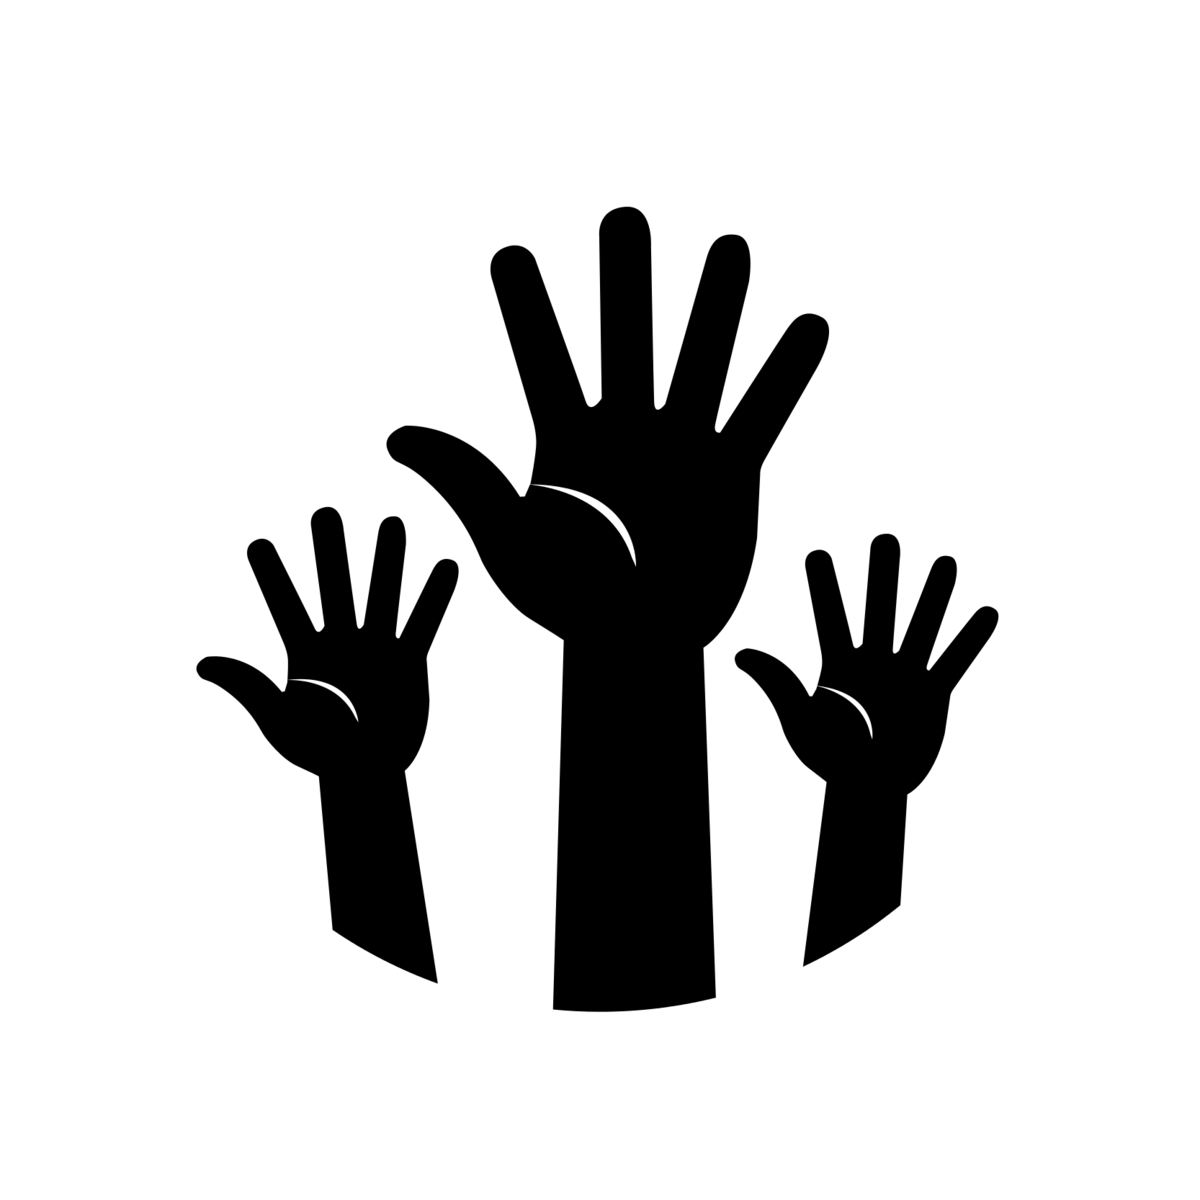
\includegraphics[height=1.5em]{images/hands}
	  	}
	  	\only<3->{
		  \begin{itemize}
		  	\item  \answer{Code \& dependencies, inputs, environment ($\rightarrow$ VM \& cloud)}
		  \end{itemize}
	  	\pause
		}
	\end{itemize}
  \medskip
	  	\pause
	
%\only<4->{
  \item We often have quite \alert{cheap} experiments
  \begin{itemize}
  	\item price for computers is monotonically decreasing
  	\item often maximal runtimes of 1h; exception: deep learning (up to a week)
  	\item compare e.g., experimental physics: 1 week of beam time per year % Still different from observing new species in the field for half a year / 
  \end{itemize}
  \smallskip
  \pause
%}
%\only<5->{
  \item We can conduct and analyze experiments fully \alert{automatically} 
  \begin{itemize}
    \item we can gather large amounts of data quickly (e.g., 100 repetitions)
  	\item but: don't confuse statistical significance and relevance
  \end{itemize}
%}	
\end{itemize}

\end{frame}
%-----------------------------------------------------------------------
%----------------------------------------------------------------------
\begin{frame}[c]{Outliers are quite different in computer experiments}

Is the following statement correct? 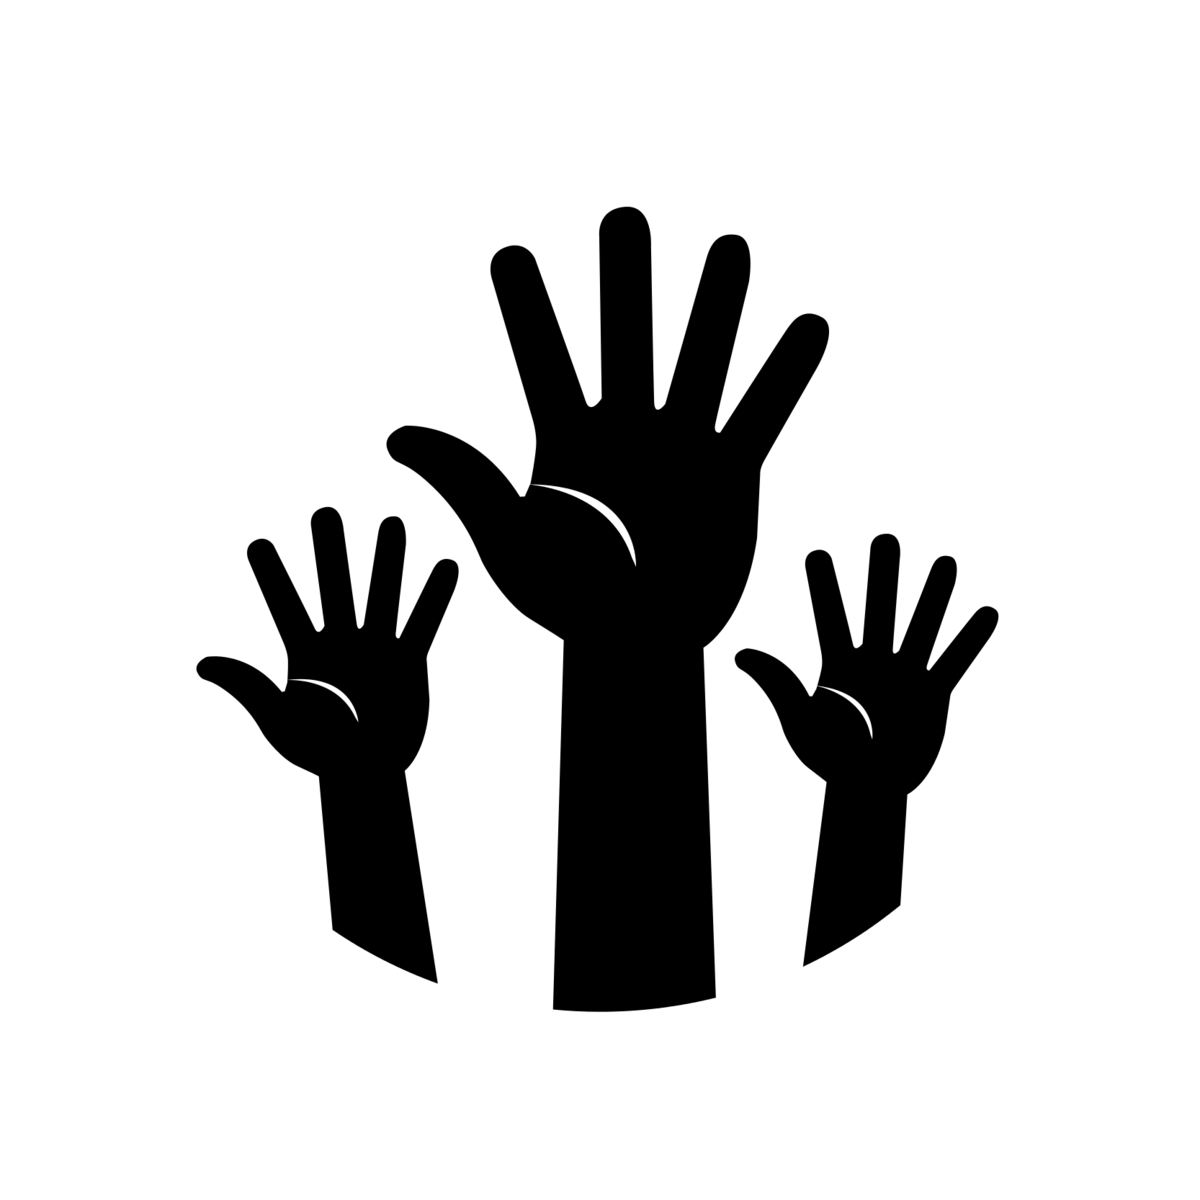
\includegraphics[height=1.5em]{images/hands}

``As usual in other empirical sciences, we (in CS) should take care to \alert{detect and remove outliers} before further analysis.''

\pause
\bigskip

\begin{block}{Outliers in CS}
\begin{itemize}
  \item outliers should be investigated closely -- why is there an outlier?
  \item outliers are (hopefully) reproducible -- narrow down their reason!
  \pause
  \begin{itemize}
    \item \textbf{Algorithm:} When characterizing runtimes of a randomized algorithm on a single instance of a hard combinatorial problem, \alert{outliers with large values can indicate deep local optima}
    \pause
    \item \textbf{Environment:} Outliers with large runtimes can indicate a \alert{problem with the runtime environment} (e.g., file system or network issues)
    \pause
    \item \textbf{Instances:}  When characterizing runtimes across a distribution of instances, outliers with small values can indicate trivial instances.
  \end{itemize}
\end{itemize}
\end{block}

\end{frame}
%-----------------------------------------------------------------------
%----------------------------------------------------------------------
\begin{frame}[c]{Application scenarios and evaluation criteria}

Evaluation criteria for algorithms depend on the application context:

\bigskip

\begin{itemize}
\item {\bf Type 1:} \alert{No time limits} 
	\begin{itemize}
		\item Algorithm can be run until a (optimal) solution is found\\(off-line computations, \eg{}, configuration of production facility)
        
        \medskip
        \item[$\leadsto$] evaluation criterion (to minimize): \alert{expected run-time}
	\end{itemize}
        
\pause
\bigskip

\item {\bf Type 2:} \alert{Hard time limit $t_{max}$} 
	\begin{itemize}
		\item Solutions found later than $t_{max}$ are useless\\
        (real-time environments with strict deadlines,\\ \eg{}, dynamic task scheduling or on-line robot control)
        
        \medskip
        \item[$\leadsto$] evaluation criterion (to maximize): \alert{solution probability at time $t_{max}$}
	\end{itemize}
\end{itemize}

\end{frame}
%-----------------------------------------------------------------------

%----------------------------------------------------------------------
\begin{frame}[c]{Application scenarios and evaluation criteria}


In many real applications, utility of solutions depends in more complex ways on time required for finding them:

\medskip

\begin{itemize}
\item {\bf Type 3:}
        Characterized by \alert{utility function $U: \Reals^+ \mapsto [0,1]$},
        where $U(t)$ = utility of solution found at time $t$.
        
  \pause
  \bigskip

	\begin{itemize}
 	  \item \emph{Example:} Direct benefit $u_0$ of solution is invariant over time, \\
        but compute time costs a fixed rate: $U(t) := u_0 - c \cdot t$
        
        \pause
        \bigskip

       \item \alert{Decision-theoretic evaluation criterion} (to maximize): \\
                {utility-weighted solution probability} $U(t) \cdot P_s(\rt \leq t)$       \\
                $\leadsto$ requires detailed knowledge of $P_s(\rt \leq t)$ for arbitrary $t$
	\end{itemize}
        
\end{itemize}

\pause
\bigskip

{\small{Note: Type 3 is a generalization of Types 1 and 2.}}% We'll show that in an exercise.}}
%\note{Let students write down $U(t)$ for type 1 and 2 scenarios.}


\end{frame}
%-----------------------------------------------------------------------



%%%%%%%%%%%%%%%%%%%%%%%%%%%%%%%%%%%%%%%%%%%%%%%%%%%%%%%%%%%%%%%%%%%%%%%%%%%%%%5555
%\section{Runtime Distributions (RTDs)}
%%%%%%%%%%%%%%%%%%%%%%%%%%%%%%%%%%%%%%%%%%%%%%%%%%%%%%%%%%%%%%%%%%%%%%%%%%%%%%5555

% ---------------------------------------------------
%\frame{
%\frametitle{Lecture Outline}
%\tableofcontents
%}
% ---------------------------------------------------


%----------------------------------------------------------------------
%\begin{frame}[c]{Runtime Distributions (RTDs)}
%
%Las Vegas algorithms are often designed and evaluated without \\
%\emph{a priori} knowledge of the application scenario; therefore:
%
%\pause
%\bigskip
%
%\begin{itemize}
%
%\item assume most general scenario:\\type 3 with unknown utility function
%       
%\pause
%\medskip
%
%\item evaluate based on solution probabilities $P_s(\rt \leq t)$ for arbitrary runtimes $t$
%
%\pause
%\bigskip
%
%\item[$\leadsto$] study distributions of \alert{random variables} characterizing the algorithm's runtime on a given problem instance
%\end{itemize}
%
%\end{frame}
%-----------------------------------------------------------------------



%----------------------------------------------------------------------
\begin{frame}[c]{Running examples of algorithms to compare}

\begin{itemize}
  \item Taken from the \alert{Configurable SAT Solver Challenge}
  \refstyle{(\url{http://aclib.net/cssc2014/})}
  \medskip
  \pause
  \item Example 1:
  \begin{itemize}
	  \item Algorithm: Lingeling \refstyle{[Biere, 2013]}
	  \begin{itemize}
	    \item[-] 2 versions: default vs.\ configured on training instances
	  \end{itemize}  
	  \pause
	  \item Benchmark set: Circuit-Fuzz \refstyle{[Brummayer et al, 2013]}
  \end{itemize}
  \bigskip
  \pause
  \item Example 2:
  \begin{itemize}
	  \item Algorithm: Clasp \refstyle{[Gebser et al, 2012]}
	  \begin{itemize}
	    \item[-] 2 versions: default vs.\ configured on training instances
	  \end{itemize}  
	  \item Benchmark set: N-Rooks \refstyle{[Manthey \& Steinke, 2014]}
  \end{itemize}
  
\pause
\medskip
  \item Comparing runtimes on \alert{test instances not used for configuration}
\end{itemize}

\end{frame}
%-----------------------------------------------------------------------


%----------------------------------------------------------------------
\begin{frame}[c]{Comparing Algorithms based on Summary Statistics}


Clasp on N-Rooks, $t_{max} = 300s$\\
\begin{tabular}{| l | l | l |}
  \hline
  ~ & Default & Configured\\
  \hline
  Average runtime [s] & $81.8$ & $4.68$\\
  PAR10 [s] & $704$ & $4.68$\\
  Timeouts (out of 351) & $81$ & $0$\\
  \hline
\end{tabular}
~\\~\\
\alert{PAR10}: penalized average runtime, counting timeouts at $t_{max}$
as $10 \cdot t_{max}$ 
~\\~\\~
\pause

Lingeling on Circuit-Fuzz, $t_{max} = 300s$\\
\begin{tabular}{| l | l | l |}
  \hline
  ~ & Default & Configured\\
  \hline
  Average runtime [s] & $47.8$ & $32.0$\\
  PAR10 [s] & $186$ & $115$\\
  Timeouts (out of 585) & $30$ & $18$\\
  \hline
\end{tabular}

%Training:
%Average runtime: $81.84 \rightarrow $
%PAR10: $704.92 \rightarrow 4.68$
%Timeouts: $81/351  \rightarrow 0/351$
\end{frame}
%-----------------------------------------------------------------------


%----------------------------------------------------------------------
\begin{frame}[c]{Runtime Distributions (RTDs)}

A typical run-time distribution for an SLS algorithm applied to a hard instance of a combinatorial decision problem:

\only<1>{
\begin{center}
\hspace*{-10mm}
\includegraphics[width=8cm]{images/hh_images_ch4/f04-01a}
\end{center}
}
\only<beamer>{
\only<2>{
\begin{center}
\hspace*{-10mm}
\includegraphics[width=8cm]{images/hh_images_ch4/f04-01a-2}
\end{center}
}
\only<3>{
\begin{center}
\hspace*{-10mm}
\includegraphics[width=8cm]{images/hh_images_ch4/f04-01a-3}
\end{center}
}
\only<4>{
\begin{center}
\hspace*{-10mm}
\includegraphics[width=8cm]{images/hh_images_ch4/f04-01a-4}
\end{center}
}
}

\end{frame}
%-----------------------------------------------------------------------


%----------------------------------------------------------------------
\begin{frame}[c]{Empirically measuring RTDs}


\begin{itemize}

\item In practice, RTDs are measured empirically 
\begin{itemize}
  \item except for very simple cases, where they can be derived analytically
 \end{itemize}
        
\pause
\medskip

\item Empirical RTDs are \alert{approximations} of an algorithm's true RTD
	\begin{itemize}
	  \item based on $N$ independent runs of the algorithm %on a given problem instance
	  \item these runs define \alert{samples of the theoretical RTD}
	  \item larger \alert{sample sizes} $N$ yield more accurate approximations 
	\end{itemize}

\end{itemize}



\end{frame}
%-----------------------------------------------------------------------

%----------------------------------------------------------------------
\begin{frame}[c]{Empirically measuring RTDs}

Typical sample of run-times for an SLS algorithm applied to an instance of a hard decision problem:

\begin{center}
\hspace*{-7mm}
\includegraphics[width=7.6cm]{images/hh_images_ch4/f04-04a}
\end{center}
\vspace*{-6mm}

\begin{itemize}
  \item Each spike is one independent run (with a different random seed)
  \item Note the high variability in runtime
\end{itemize}


\end{frame}
%-----------------------------------------------------------------------

%----------------------------------------------------------------------
\begin{frame}[c]{Empirically measuring RTDs}

\begin{multicols}{3}
\vspace*{2.5cm}
\includegraphics[width=4.0cm]{images/hh_images_ch4/f04-04a}
%\columnbreak$\xrightarrow[]{\text{sort by runtimes}}$ \\~\\~\\~\\~\\~\\~\\~\\~\\~\\~\\~\\~\\~\\~\\~\\~\\~\\~\\~\\
\columnbreak
\vspace*{1.0cm}
~~~~~~\\~~~~~~\includegraphics[width=4.0cm,angle=90,origin=c]{images/hh_images_ch4/f04-04b}
\columnbreak
~~
\\\includegraphics[width=4.0cm,origin=c]{images/hh_images_ch4/f04-04b}\\
\begin{center}
Corresponding empirical RTD
\end{center}
\end{multicols}

\vspace*{-0.2cm}
\begin{itemize}
  \item Sort by runtimes
  \item Rotate
\end{itemize}

\end{frame}
%-----------------------------------------------------------------------


%----------------------------------------------------------------------
\begin{frame}[c]{Empirically measuring RTDs}


Corresponding empirical RTD:

\begin{center}
\hspace*{-13mm}
\includegraphics[width=7.6cm]{images/hh_images_ch4/f04-04b}
\end{center}

\end{frame}
%-----------------------------------------------------------------------
%----------------------------------------------------------------------
\begin{frame}[c]{Comparing algorithms based on their runtime distributions}

\begin{center}
\includegraphics[height=6cm]{scripts/runtime_plots/cdf_test_clasp_queens.png}\\~\\
\vspace*{-0.3cm}
Distributions of runtime \alert{across benchmark instances}\\
(Clasp on N-Rooks) %(351 test instances)
\end{center}

\end{frame}
%-----------------------------------------------------------------------

%----------------------------------------------------------------------
\begin{frame}[c]{Comparing algorithms based on their runtime distributions}

\begin{center}
\includegraphics[height=6cm]{scripts/runtime_plots/cdf_test_lingeling_circuitfuzz.png}\\~\\
\vspace*{-0.3cm}
~\\
(Lingeling on Circuit-Fuzz) %(585 test instances)
\end{center}

\end{frame}
%-----------------------------------------------------------------------




%----------------------------------------------------------------------
\begin{frame}[c]{Comparing algorithms based on scatter plots}

\begin{center}
\includegraphics[height=6cm]{scripts/runtime_plots/scatter_test_clasp_queens}\\~\\
\vspace*{-0.5cm}
Each marker represents one instance; note the \alert{log-log axis}!\\
\vspace*{0.2cm}
(Clasp on N-Rooks; 81 vs.\ 0 timeouts)
 
\end{center}

\end{frame}
%-----------------------------------------------------------------------

%----------------------------------------------------------------------
\begin{frame}[c]{Comparing algorithms based on scatter plots}

\begin{center}
\includegraphics[height=6cm]{scripts/runtime_plots/scatter_test_lingeling_circuitfuzz.png}\\~\\
\vspace*{-0.5cm}
~\\
\vspace*{0.2cm}
(Lingeling on Circuit-Fuzz; 30 vs.\ 18 timeouts)
\end{center}

\end{frame}
%-----------------------------------------------------------------------



%----------------------------------------------------------------------
\begin{frame}[c]{Comparing algorithms based on scatter plots}

Scatter plots can reveal clear patterns in the data

\begin{multicols}{2}
\begin{center}
\includegraphics[height=5cm]{images/CSSC_Results/SparrowToRiss-K3-300-scatter_test.png}
\end{center}
\columnbreak
~\\
Example: an algorithm in default mode that
\begin{itemize}
  \item first runs algorithm A\\(good for satisfiable instances)\\for $t$ seconds
  \item then runs algorithm B (good for unsatisfiable instances) until time is up 
\end{itemize} 
\end{multicols}
\vspace*{-0.2cm}

\begin{center}

\pause
\smallskip
There are 2 instance clusters: satisfiable and unsatisfiable instances\\
\vspace*{0.1cm}
Which cluster is which? \raisebox{-0.2cm}{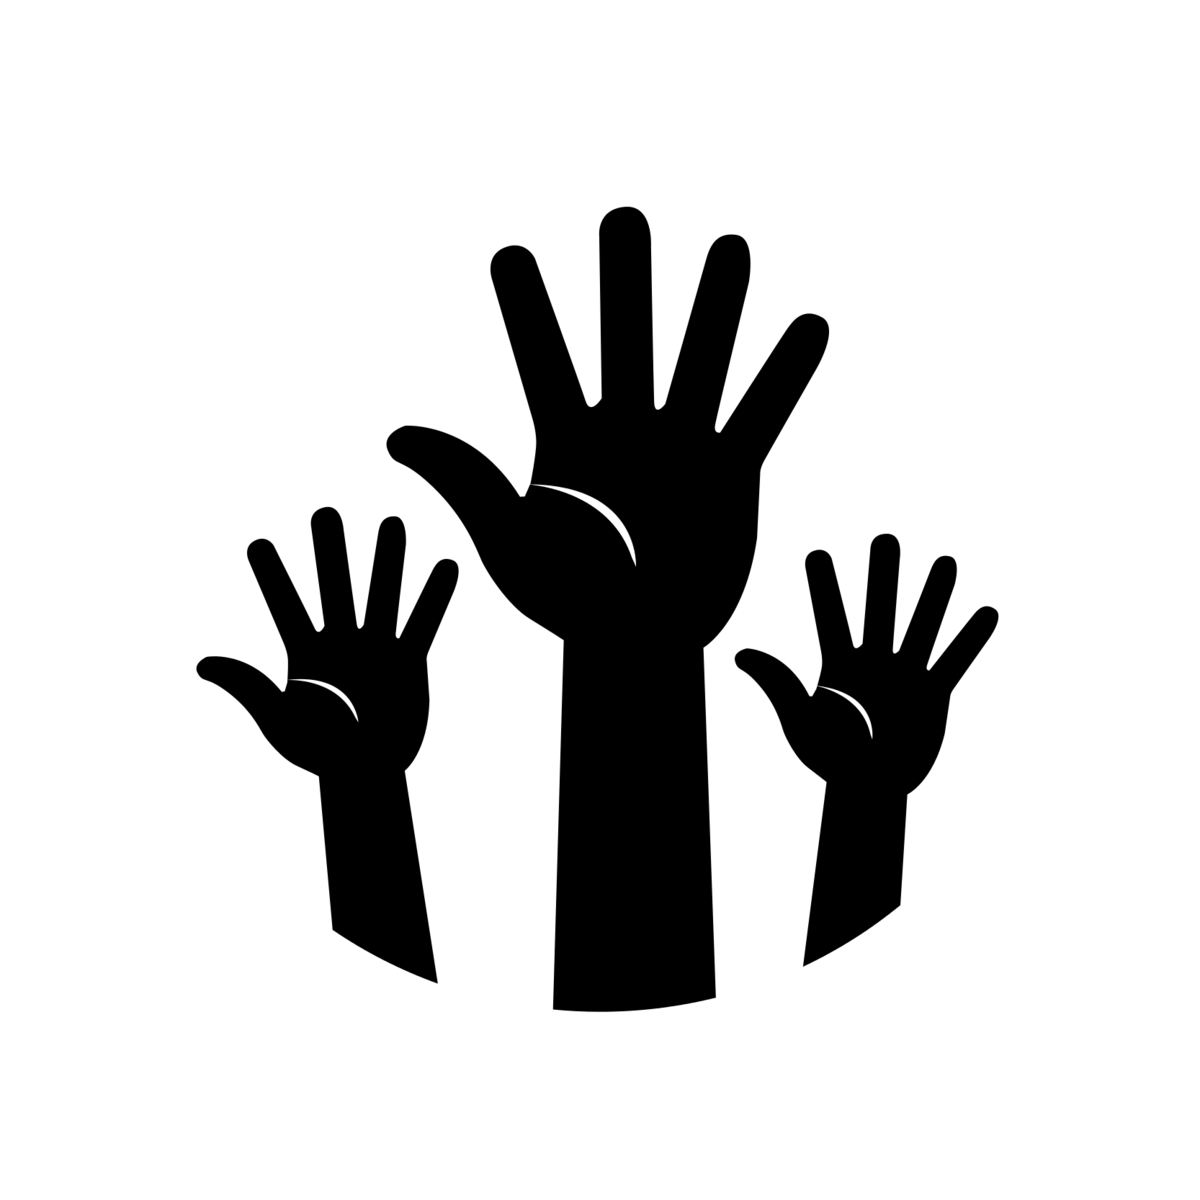
\includegraphics[height=0.6cm]{images/hands}}\\
%\vspace*{0.1cm}
%\pause Satisfiable instances are ~\voteblue{} left ~ \voteyellow{} right
\end{center}

%Average Runtime	19.75	9.53
%PAR10	52.15	9.53
%Timeouts	3 / 250	0 / 250


\end{frame}
%-----------------------------------------------------------------------


%----------------------------------------------------------------------
\begin{frame}[c]{Comparing algorithms with boxplots (box-and-whisker plot)}

\vspace*{-0.5cm}
\begin{center}
\includegraphics[height=5cm]{scripts/runtime_plots/crafted_CSSC-Queens-300s-2day_clasp-3_0_4-p8_paramils-2_TEST_csv_boxplot.pdf}~
\includegraphics[height=4cm]{scripts/runtime_plots/scatter_test_clasp_queens}\\~\\
\vspace*{-0.3cm}
Box: 25\% quantile -- 75\% quantile; red line: median\\
Dashed line to ends of ranges, outliers as `+' symbols\\~\\
\pause
Note the wide variation (due to instance hardness)!\\
Visually not obvious that \emph{configured} performs much better than
\emph{default}
\end{center}

\end{frame}
%-----------------------------------------------------------------------


%----------------------------------------------------------------------
\begin{frame}[c]{Comparing algorithms with boxplots (box-and-whisker plot)}

\vspace*{-0.5cm}
\begin{center}
\includegraphics[height=5cm]{scripts/runtime_plots/crafted_CSSC-Queens-300s-2day_clasp-3_0_4-p8_paramils-2_TEST_csv_boxplot_ratio.pdf}~
\includegraphics[height=4cm]{scripts/runtime_plots/scatter_test_clasp_queens}\\~\\
\vspace*{-0.3cm}
\alert{Ratio} of \emph{default} and \emph{configured} runtime\\ (distribution of that ratio across instances) \pause\\~\\
Now most points lie above 1 $\rightarrow$ \emph{configured} better on almost all instances 
\end{center}

\end{frame}
%-----------------------------------------------------------------------



%----------------------------------------------------------------------
\begin{frame}[c]{Comparing algorithms with boxplots (box-and-whisker plot)}

\vspace*{-0.5cm}
\begin{center}
\includegraphics[height=5cm]{scripts/runtime_plots/industrial_CSSC-CircuitFuzz-300s-2day_lingeling_paramils-1_TEST_csv_boxplot.pdf}~
\includegraphics[height=4cm]{scripts/runtime_plots/scatter_test_lingeling_circuitfuzz.png}\\~\\
\vspace*{-0.3cm}

(Lingeling on Circuit-Fuzz)
\end{center}

\end{frame}
%-----------------------------------------------------------------------


%----------------------------------------------------------------------
\begin{frame}[c]{Comparing algorithms with boxplots (box-and-whisker plot)}

\vspace*{-0.5cm}
\begin{center}
\includegraphics[height=5cm]{scripts/runtime_plots/industrial_CSSC-CircuitFuzz-300s-2day_lingeling_paramils-1_TEST_csv_boxplot_ratio.pdf}~
\includegraphics[height=4cm]{scripts/runtime_plots/scatter_test_lingeling_circuitfuzz.png}\\~\\
\vspace*{-0.3cm}
\alert{Ratio} of \emph{default} and \emph{configured} runtime\\
(Lingeling on Circuit-Fuzz)
\end{center}

\end{frame}
%-----------------------------------------------------------------------


%----------------------------------------------------------------------
\begin{frame}[c]{Algorithm Footprints~\litw{Smith-Miles et al.}}

\begin{block}{Idea}
Visualize performance in instance space (not in performance space!)
\begin{enumerate}
  \item Use PCA to project instance features in 2d
  \item Mark all instances for which algorithm $\algo$ performs similar as oracle
\end{enumerate}
\end{block}

\begin{center}
\includegraphics[height=5cm]{images/footprint_march_rw_2011-03-02}
\end{center}

\end{frame}
%-----------------------------------------------------------------------




% ---------------------------------------------------
%----------------------------------------------------------------------
\begin{frame}[c]{Background: statistical hypothesis tests}

\begin{itemize}
  \item When we have a lot of data, we need to summarize it
  \begin{itemize}
	  \item But we already saw that summarization hides a lot of data
%	  \item E.g., a single outlier might explain the difference in means
	  \item Ideally, we want to draw high-level conclusions\\
	  (e.g., ``A outperforms B on instances of type X'')
  \end{itemize}

\pause
\bigskip

  \item Problem: we only have a finite number of observations
  \begin{itemize}
	  \item Can we attribute observed performance differences to chance?
	  \item Are we reasonably sure that a claim we make is reproducible?
	  \item[$\leadsto$] Statistical tests can help
  \end{itemize}


\end{itemize}

\medskip

\end{frame}
%-----------------------------------------------------------------------
%----------------------------------------------------------------------
\begin{frame}[c]{Statistical hypothesis testing}

\begin{enumerate}
  \item Define initial research hypothesis
  \pause
  \item Derive null $H_0$ and alternative $H_1$ hypothesis
  \begin{itemize}
    \item Alternative hypothesis should be your research hypothesis
  \end{itemize}
  \pause
\end{enumerate}	

\end{frame}
%-----------------------------------------------------------------------
%----------------------------------------------------------------------
\begin{frame}[c]{First example: Courtroom Tiral}

\begin{itemize}
	\item A prosecutor tries to prove the guilt of the defendant
	\item $H_0$: 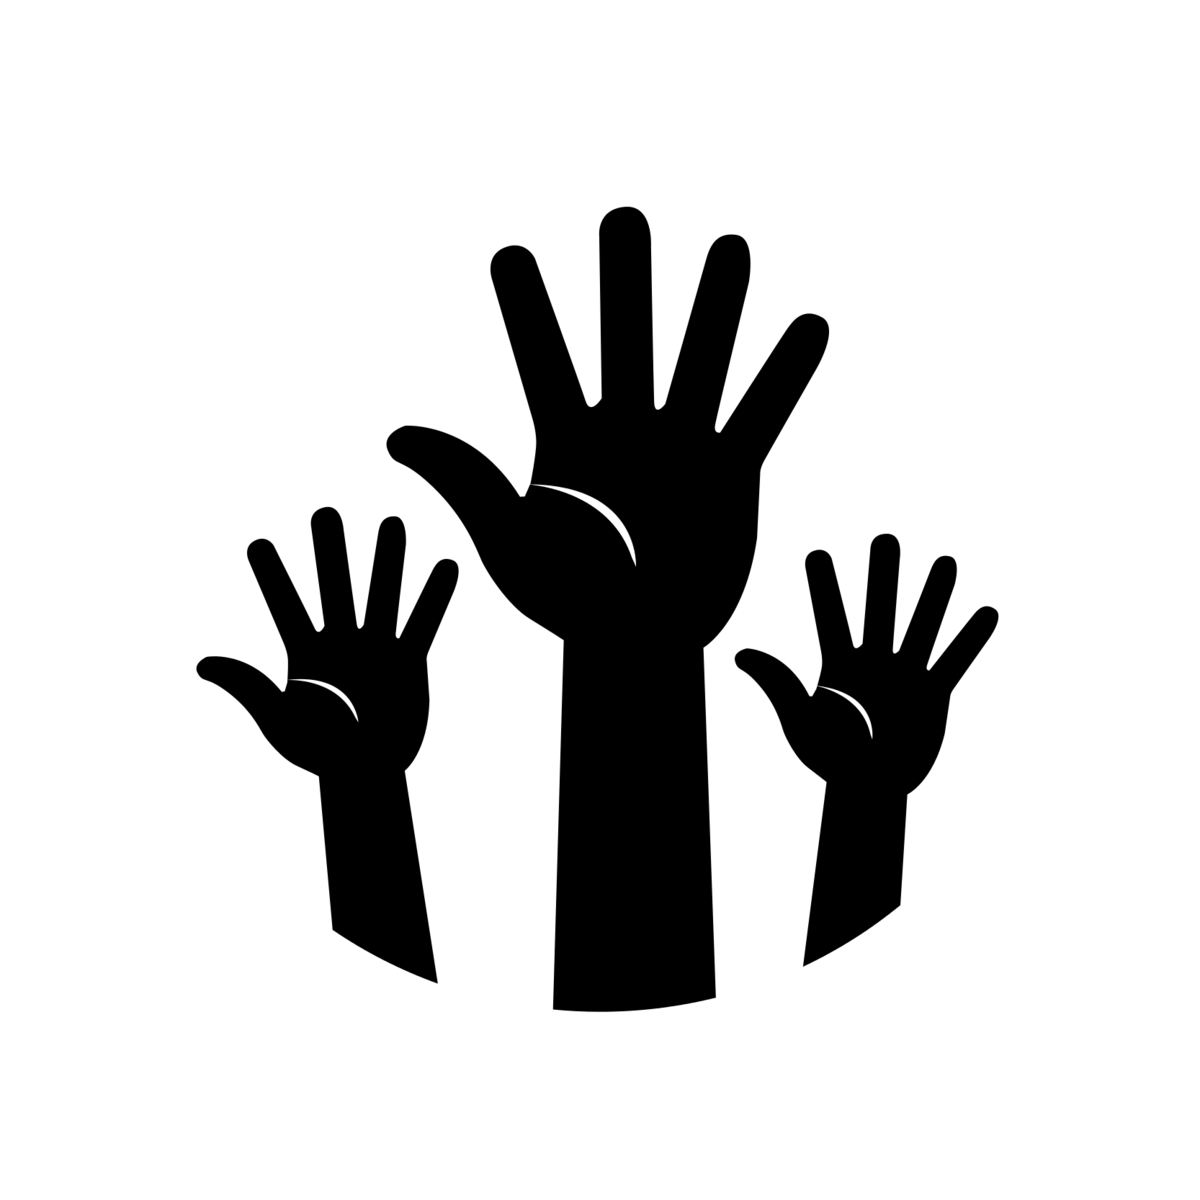
\includegraphics[height=1em]{images/hands} \only<2->{The defendant is not guilty
	\begin{itemize}
	  \item Accepted for the moment\\ (``not guilty as long as their guilt is not proven'') 
	\end{itemize}
	}
	\item $H_1$: 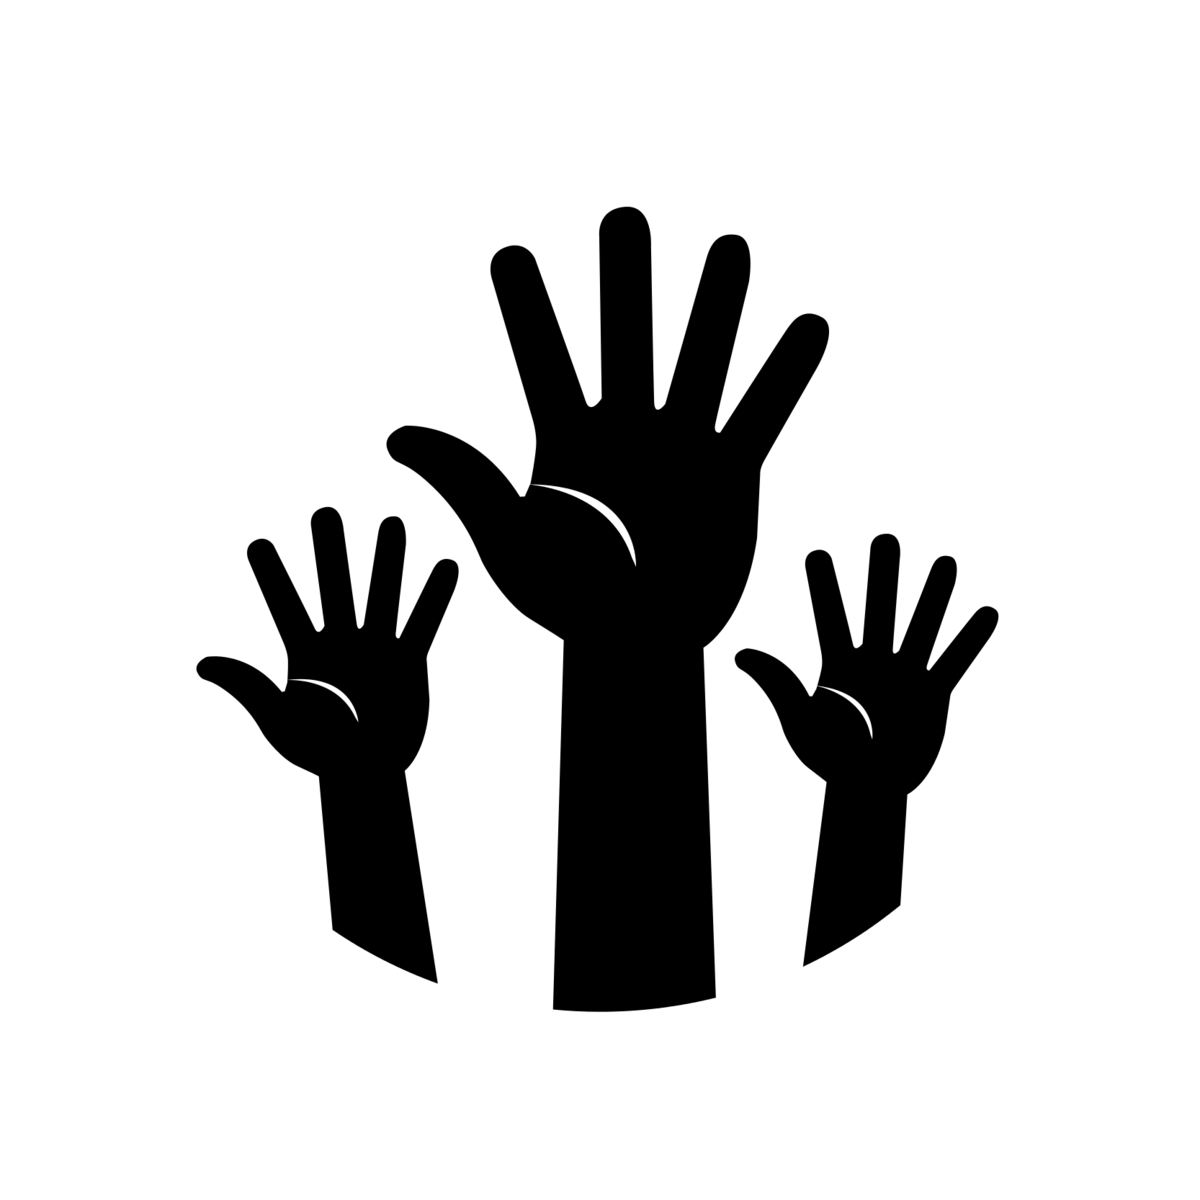
\includegraphics[height=1em]{images/hands} \only<2->{The defendant is guilty
	\begin{itemize}
	  \item prosecutor hopes to support that
	\end{itemize}
	}
	\pause
\end{itemize}

\medskip
\pause
\bigskip
\centering
\begin{tabular}{c|cc}
\toprule
 			& Truly not guilty 	& Truly guilty\\
 \hline
 Acquittal 	& Right decision	& Type II Error\\
 Conviction & Type I Error		& Right decision\\
\bottomrule
\end{tabular}	

\bigskip
$\leadsto$ We want to minimize Type I error!

\end{frame}
%-----------------------------------------------------------------------
%----------------------------------------------------------------------
\begin{frame}[c]{Statistical hypothesis testing (cont'd)}

\begin{enumerate}
  \item Define initial research hypothesis
  \item Derive null $H_0$ and alternative $H_1$ hypothesis
  \begin{itemize}
    \item Alternative hypothesis should be your research hypothesis
  \end{itemize}
  \item Consider statistical assumptions
  \begin{itemize}
    \item E.g., is your data Gaussian distributed?
  \end{itemize}
  \pause
  \item Decide test and test statistic $T$
  \begin{itemize}
    \item The correct test depends on your statistical assumptions.
    \item Typically: if you use more assumptions, the test is more powerful\\ (i.e., less Type-I error)
  \end{itemize}
  \pause
  \item Decide significance level $\alpha$\\ (i.e., acceptable Type-I error to reject null hypothesis)
  \pause
  \item Compute observed $t_{obs}$ of test statistic $T$
  \item Calculate $p$-value given $t_{obs}$
  \begin{itemize}
    \item i.e., probability under the null hypothesis of sampling a test statistic as extreme as observed (probability of Type-I error)
  \end{itemize} 
  \pause
  \item If $p < \alpha$, reject null hypothesis in favor of alternative hypothesis
  \begin{itemize}
    \item If $p > \alpha$, it doesn't tell you anything about the null hypothesis!
  \end{itemize}
\end{enumerate}	

\end{frame}
%-----------------------------------------------------------------------
%----------------------------------------------------------------------
\begin{frame}[c]{Second example for a statistical test}

\begin{itemize}
  \item IQ values are known to be normally distributed with $X \sim
  \mathcal{N}(100,15)$
  \begin{itemize}
    \item$\to$ statistical assumption
  \end{itemize}
  % \\with mean $100$ and variance $15$: $X \sim \mathcal{N}(100,15)$
  \item Claim: \alert{``the students in this class are more intelligent
  than average''}
  \bigskip
  \pause
  \item \alert{Null Hypothesis $H_0$}: $\mu=100$ ($\mu$ is the population
  mean of this class)
  \item \alert{Alternative Hypothesis $H_1$}: $\mu>100$ (\alert{one-sided} hypothesis)

\bigskip
\pause

  \item Let's say we observed IQ values $x_i$ of 9 students in the class:
    \begin{itemize}
	  \item $\{x_1,\dots,x_9\} = \{116, 128, 125, 119, 89, 99, 105, 116, 118\}$.
	  \item The \alert{sample mean} is $\bar{x}=112.8$
	  \item Does this data support the claim?
	\end{itemize}	

\end{itemize}	

\end{frame}
%-----------------------------------------------------------------------


%----------------------------------------------------------------------
\begin{frame}[c]{Example continued}

\begin{itemize}

  \item \alert{Distribution of the test statistic} 
  \begin{itemize}
	  \item Under $H_0$, we know that each $x_i \sim \mathcal{N}(100,15)$
	  \smallskip
	  \item The \alert{test statistic} that we measure is the sample
	  mean $\bar{x} = \frac{1}{9} \sum_{i=1}^9 x_i$
%    \item[-] $\bar{x} \sim  \mathcal{N}(\mu=100,\sigma^2=15/\sqrt{n})=\mathcal{N}(100,5)$
	  \bigskip
	  \pause
	  \item Under $H_0$, the distribution of $\bar{x}$ is
	  $\mathcal{N}(100,15/\sqrt{9})$
	  \begin{itemize}
	    \item[-] Our observation $\bar{x}=112.8$ is quite extreme under that
	    distribution
	  \end{itemize}
	\end{itemize}	
\end{itemize}

\begin{center}
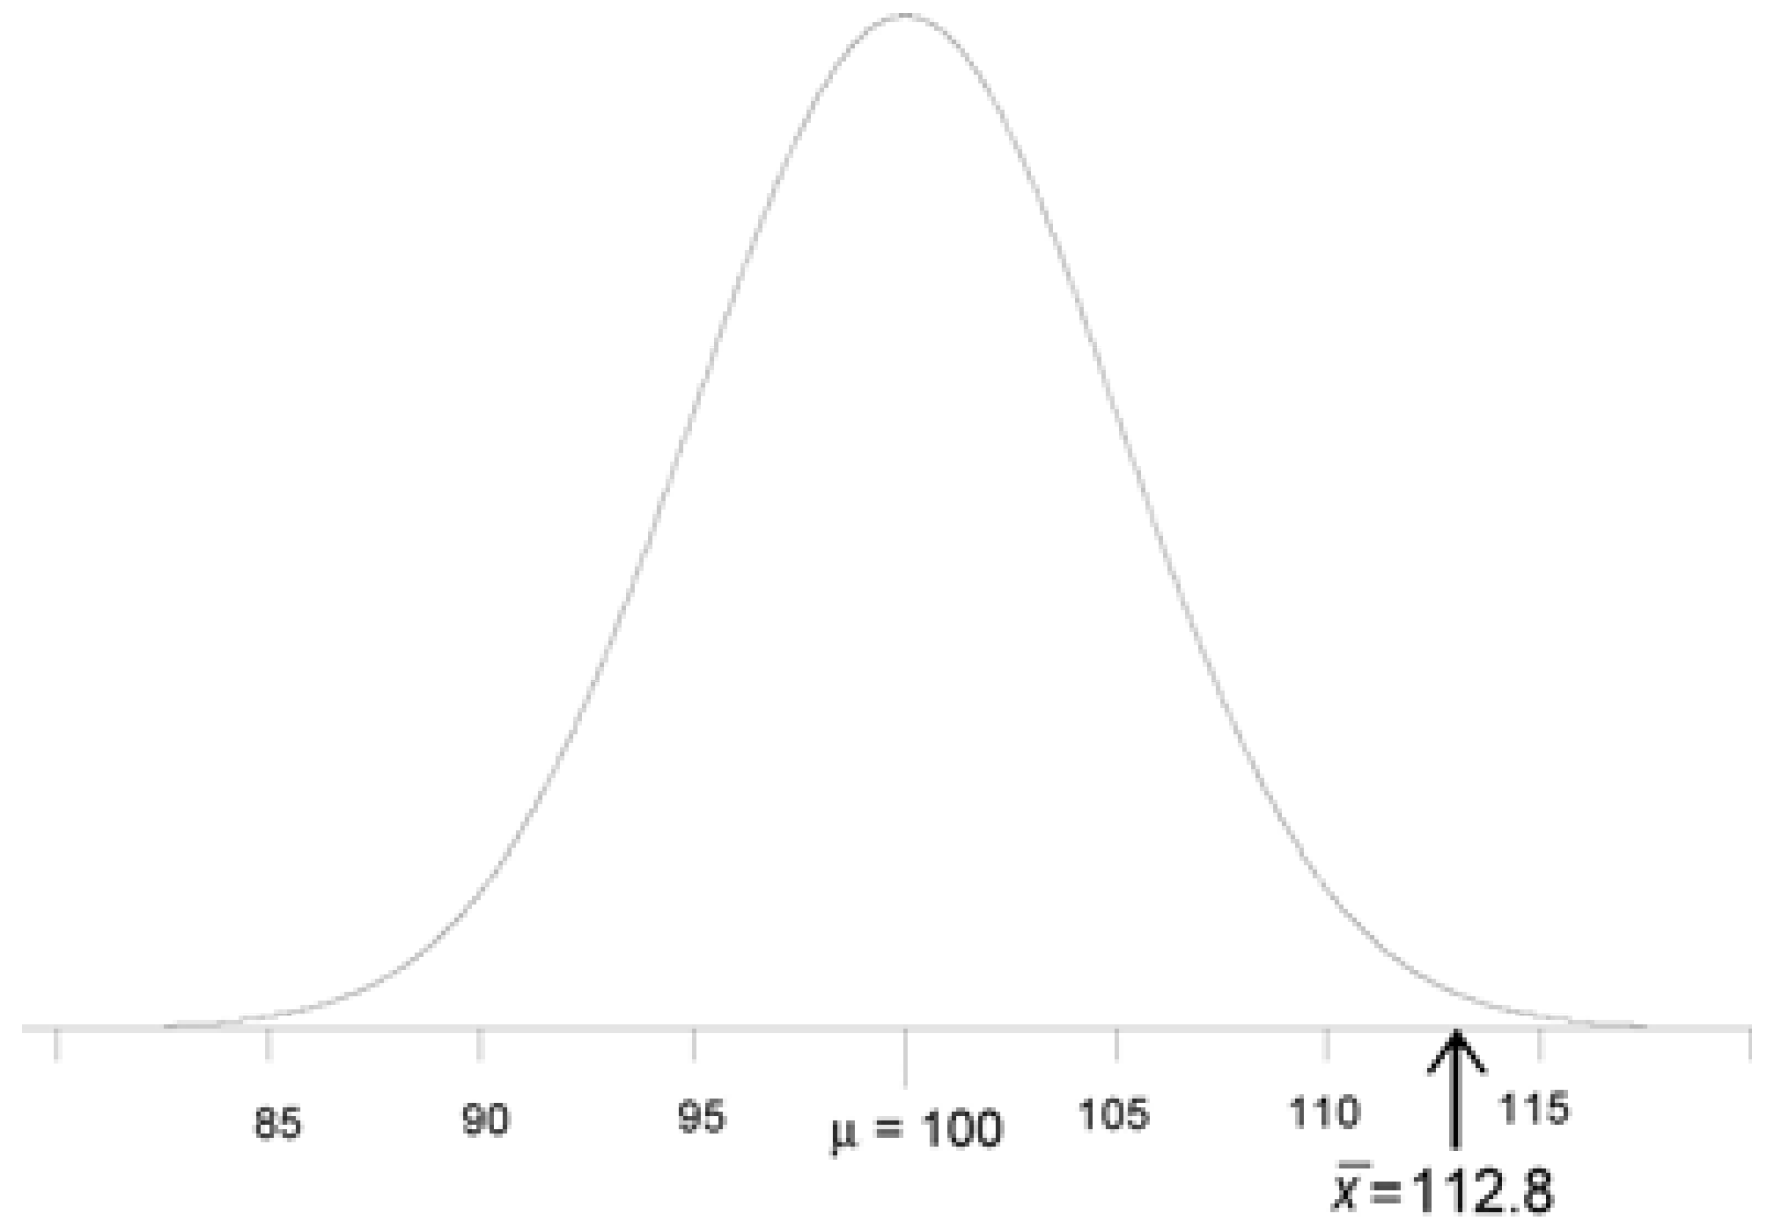
\includegraphics[height=3cm]{images/z_test_1.png}
\end{center}

\end{frame}
%-----------------------------------------------------------------------

%----------------------------------------------------------------------
\begin{frame}[c]{General principle}

\vspace*{-0.2cm}
\begin{center}
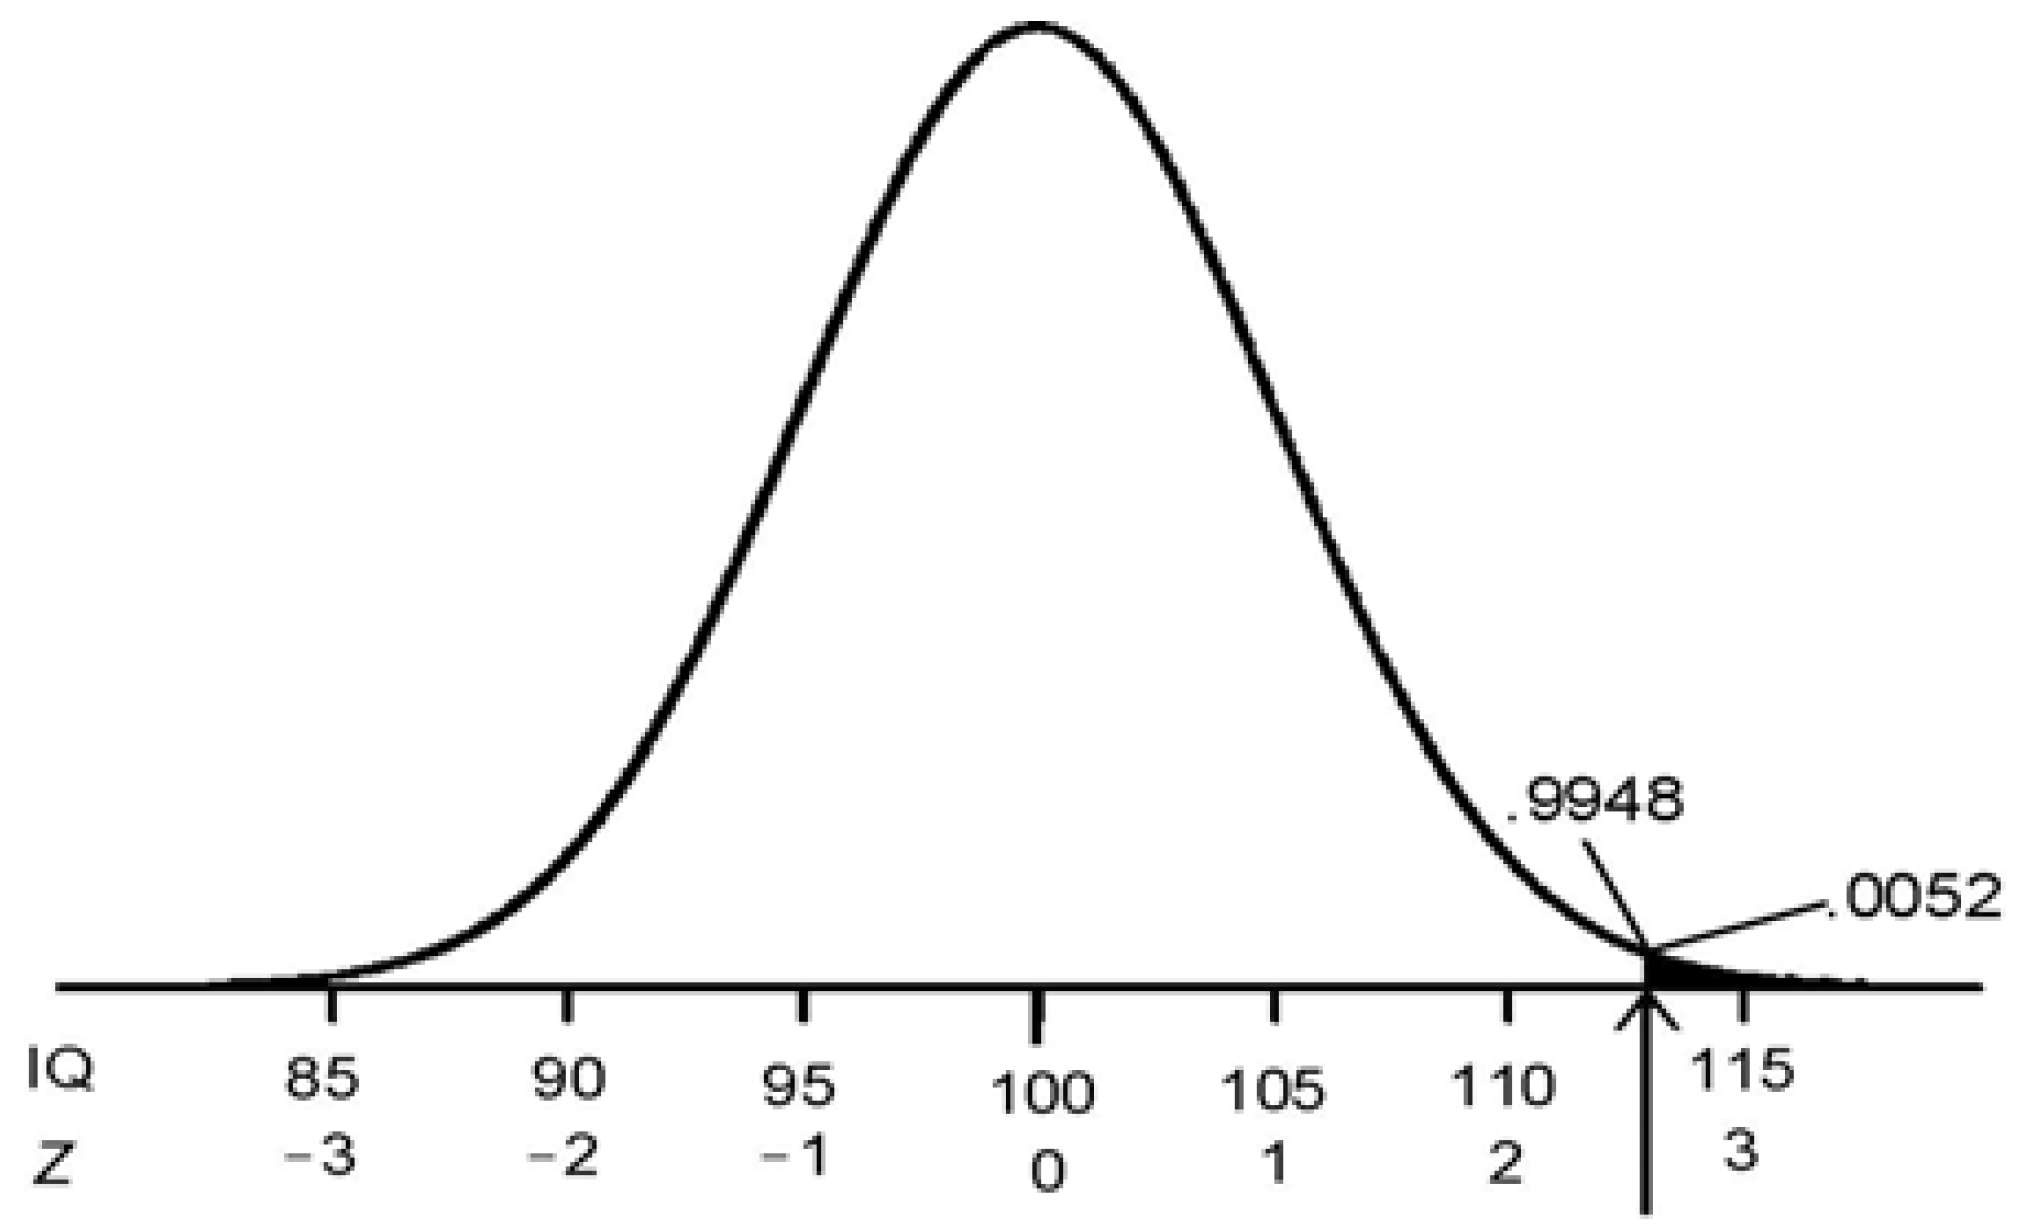
\includegraphics[height=3cm]{images/z_test_2.png}
\end{center}
\vspace*{-0.2cm}

\begin{itemize}
  \item Compare the test statistic (here: $\bar{x}$)\\to its sampling
  distribution under $H_0$
 \pause 
\medskip
  \item \alert{P-value}: probability $p$ of observing values \alert{at least as extreme as $\bar{x}$}\\
%  $\leadsto$ this is the %(computed through cumulative distribution function)
 \pause 
\medskip
  \item Compare $p$ to pre-defined confidence level $\alpha$ (usually
  $\alpha=0.05$);\\\alert{if $p < \alpha$, reject $H_0$}
 \pause 
\medskip
  \item With $\alpha = 0.01$, would we reject $H_0$ in this case? \hands
\end{itemize}

\end{frame}
%-----------------------------------------------------------------------


%----------------------------------------------------------------------
\begin{frame}[c]{Summary of example}

\begin{itemize}
  \item We just used a so-called \alert{$Z$-test}
  \item $H_0$: $\mu=\mu_0$, $H_1$: $\mu>\mu_0$  
  \item Assumptions: $X \sim \mathcal{N}(\mu,\sigma^2)$ , with known $\mu$ and $\sigma^2$
    
\medskip
\pause
  \item \alert{Test statistic}: sample mean $\bar{x}$; evaluate under 
  $\mathcal{N}(\mu=\mu_0,s=\sigma^2/\sqrt{n})$
  \pause
  \smallskip
  \item Equivalent: compute the \alert{Z-statistic}: $Z = (\bar{x}-\mu_0)/s$
  and\\
  evaluate cumulative density $\Phi(Z)$ of $Z$
  under $\mathcal{N}(0,1)$
\medskip
\pause
  \begin{itemize}
    \item There are standard tables to look up $\Phi(Z)$ for different values of $Z$
    \item Nowadays, there are standard libraries to compute $\Phi(Z)$
  \end{itemize}
    
\end{itemize}

\end{frame}
%-----------------------------------------------------------------------


%----------------------------------------------------------------------
\begin{frame}[c]{Two-sided tests}


\vspace*{-0.2cm}
\begin{center}
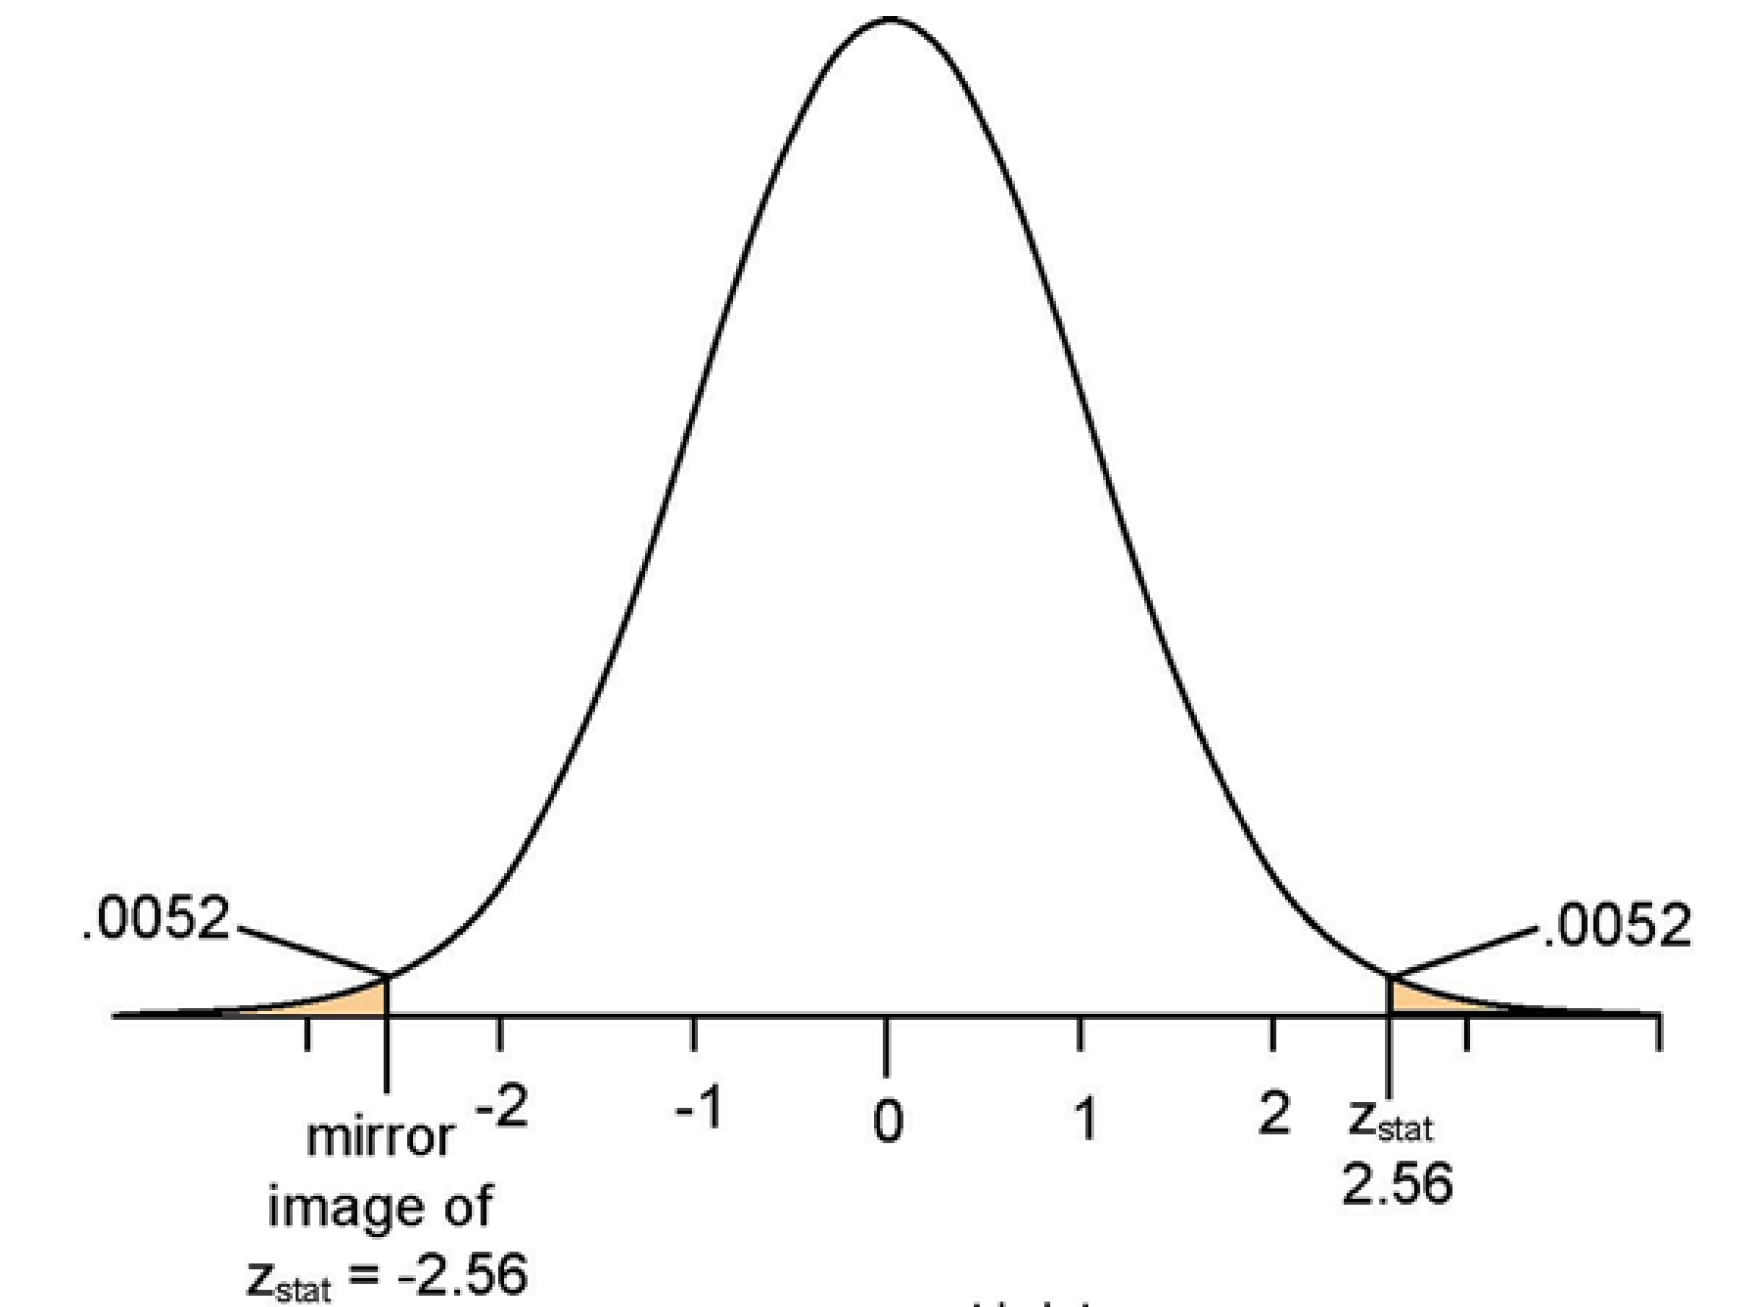
\includegraphics[height=3.5cm]{images/z_test_3.png}
\end{center}
\vspace*{-0.2cm}

\begin{itemize}
  \item Similar to one-sided tests, but testing for extreme values in both tails
  \item Example Z-test: two-sided alternative hypothesis $H_1$:
  $\mu \neq \mu_0$
  \pause
  \smallskip
  \item Compute $Z = (\bar{x}-\mu_0)/s$ as before
  \item Compute $p$-value as $p = 2\Phi(Z)$, to account for both tails
 \pause 
\medskip
  \item With $\alpha = 0.01$, would we reject $H_0$ in this case? \hands
\end{itemize}

\end{frame}
%-----------------------------------------------------------------------


%----------------------------------------------------------------------
\begin{frame}[c]{General points about statistical hypothesis tests}

\begin{itemize}
  \item What if $p > \alpha$?
  \begin{itemize}
	  \item \alert{Failure to reject $H_0$}
	  \item \alert{This does not mean that we accept $H_0$}
  \end{itemize}


\pause
\bigskip
  \item Beware: most tests make some assumptions
  \begin{itemize}
	  \item E.g., $Z$-test and popular $t$-test assume \alert{normality}
	  \item Our data is often far from normally-distributed
	  \begin{itemize}
	    \item[$\leadsto$] E.g., exponential runtime distributions of SLS solvers for SAT
	    \item[$\leadsto$] E.g., distribution of fitting a neural network\\ with different random seeds is not well studied
	  \end{itemize}
  \end{itemize}

\end{itemize}

\end{frame}
%-----------------------------------------------------------------------


%----------------------------------------------------------------------
\begin{frame}[c]{The permutation test: a better test for non-normal data}

\begin{itemize}
  \item Framework for testing several types of claims
  \item E.g., $H_0$: $X$ and $Y$ have \alert{equal means}
  \item Test statistic: \alert{$t = \frac{1}{n}\sum_{i=1}^n x_i  - 
  \frac{1}{m}\sum_{j=1}^m y_j$}
  \pause
  \medskip
  \item The sampling distribution to compare $t$ against:
  \begin{itemize}
    \item Put $x_1, \dots, x_n$ and $y_1, \dots, y_m$ into a single pool
    \item S = []; repeat, e.g., 10\,000 times
    \begin{itemize}
      \item[-] draw a random permutation \& permute pool with it
      \item[-] add test statistic over permuted pool to $S$
    \end{itemize}
  \end{itemize}
  \pause
  \medskip
  \item $p$-value: percentile of $s$ in $S$:\\
  fraction of samples $s$ in $S$ with $s < t$

\end{itemize}

\end{frame}
%-----------------------------------------------------------------------

\hide{
%----------------------------------------------------------------------
\begin{frame}[c]{The Wilcoxon rank-sum test for non-normal data}

  \begin{itemize}
    \item Compare the distributions of random variables $X$ and $Y$ 
    \begin{itemize}
      \item[-] based on samples $x_1, \dots, x_n$ and $y_1, \dots, y_m$
    \end{itemize}
\smallskip
    \item Assumptions
    \begin{itemize}
      \item[-] All of $x_1, \dots, x_n$ and $y_1, \dots, y_m$ are independent
      from each other 
      \item[-] Responses are ordinal (we can compare them)
    \end{itemize}  
    \pause
    \item $H_0$: $P(X > Y) = P(Y > X)$
    \pause
    \item $H_1$: $P(X > Y) > P(Y > X)$ (one-sided)
    \medskip
    \pause
    \item Test statistic
    \begin{itemize}
      \item[-] Order all elements $x_i$ and $y_j$ and give them ranks
    (1 for smallest)
      \item[-] Compute the sum of ranks of $x_i$ and of $y_j$
\smallskip
\pause
    \end{itemize}
    \item Under $H_0$, the distribution of that test statistic is known\\
      $\leadsto$ can evaluate how extreme the observed test statistic is
  \end{itemize}

\end{frame}
%-----------------------------------------------------------------------
}


%----------------------------------------------------------------------
\begin{frame}[c]{Example for Permutation test}

\begin{center}
\includegraphics[height=4cm]{scripts/runtime_plots/crafted_CSSC-Queens-300s-2day_clasp-3_0_4-p8_paramils-2_TEST_csv_boxplot.pdf}~
\includegraphics[height=3cm]{scripts/runtime_plots/scatter_test_clasp_queens}\\~\\
\vspace*{-0.3cm}
\end{center}

\begin{itemize}
  \item $X$: runtime of \emph{configured} on a random instance; $Y$: of  \emph{default}
  \item Data: $x_1, \dots, x_{351}$ vs.\ $y_1, \dots, y_{351}$
\pause
  \item Based on all 351 instances: $p = 0.0000$
\pause
  \item Based on just first 10 instances: $p = 0.073$  
\end{itemize}

\end{frame}
%-----------------------------------------------------------------------

%----------------------------------------------------------------------
\begin{frame}[c]{Paired vs.\ unpaired tests}

\begin{center}
\includegraphics[height=4cm]{scripts/runtime_plots/crafted_CSSC-Queens-300s-2day_clasp-3_0_4-p8_paramils-2_TEST_csv_boxplot_ratio.pdf}~
\includegraphics[height=3cm]{scripts/runtime_plots/scatter_test_clasp_queens}\\~\\
\vspace*{-0.7cm}
\end{center}

\begin{itemize}
  \item Data sometimes comes in pairs
  \item Here: We have runtimes $x_i$ and $y_i$ for the \alert{same} instance
  \item \alert{Paired statistical tests} take this pairing into account 
\pause
  \item Paired version of permutation test
  \begin{itemize}
    \item[-] Similar to unpaired version, but permute pools $\{x_i,y_i\}$ for all $i$
    \item[-] Based on just first 10 instances: $p = 0.0000$  (vs.\ 0.073 for
    rank-sum)
  \end{itemize}
\end{itemize}

\end{frame}
%-----------------------------------------------------------------------

%----------------------------------------------------------------------
\begin{frame}[c]{Cost over Time}

\begin{itemize}
  \item All algorithms run for some time $t$
  \item What would happen if we terminate it after $t' \leq t$?
  \item Time limits are arbitrary 
  \item[$\leadsto$] better to compare \emph{anytime} performance of algorithms
  \begin{itemize}
    \item most optimization algorithms are anytime algorithms
  \end{itemize}
\end{itemize}

\pause

\begin{center}
\includegraphics[height=5.5cm]{images/sklearn_over_time}~
\end{center}


\end{frame}

\hide{
%----------------------------------------------------------------------
\begin{frame}[c]{Permutation test}

\begin{itemize}
  \item Framework for testing several types of claims
  \item E.g., $H_0$: $X$ and $Y$ have \alert{equal means}
  \item Test statistic: \alert{$t = \frac{1}{n}\sum_{i=1}^n x_i  - 
  \frac{1}{m}\sum_{j=1}^m y_j$}
  \pause
  \item The sampling distribution to compare $t$ against:
  \begin{itemize}
    \item[-] Put $x_1, \dots, x_n$ and $y_1, \dots, y_m$ into a single pool
    \item[-] S = []; repeat, e.g., 10\,000 times
    \begin{itemize}
      \item[+] draw a random permutation \& permute pool with it
      \item[+] add test statistic over permuted pool to $S$
    \end{itemize}
  \end{itemize}
  \pause
  \item $p-value$: fraction of samples $s$ in $S$ with $s < t$

\end{itemize}

\end{frame}
%-----------------------------------------------------------------------
}


\hide{
%----------------------------------------------------------------------
\begin{frame}[c]{A runtime distribution for combinatorial optimization}

\begin{center}
\hspace*{-10mm}
\only<1>{%
\includegraphics[width=8cm]{images/hh_images_ch4/f04-01b}
}%
\only<beamer>{%
\only<2>{%
\includegraphics[width=8cm]{images/hh_images_ch4/f04-01b-2}
}%
\only<3>{%
\includegraphics[width=8cm]{images/hh_images_ch4/f04-01b-3}
}%
}%
\end{center}

\end{frame}
%-----------------------------------------------------------------------


%----------------------------------------------------------------------
\begin{frame}[c]{Qualified runtime distributions for various solution qualities}

\vspace*{3mm}

\begin{center}
\hspace*{-10mm}
\includegraphics[height=5cm]{images/hh_images_ch4/f04-02a}
\end{center}


\end{frame}
%-----------------------------------------------------------------------
}

%----------------------------------------------------------------------
\begin{frame}[c]{Running example: stochastic gradient descent (SGD)}

\begin{itemize}
  \item Most machine learning models internally optimize $n$ weights
  \medskip
  \pause
  \item Stochastic gradient descent (SGD) is very popular for this problem
  \medskip
  \pause
  \item \alert{Gradient descent} is just like local search:
  \begin{itemize}
    \item Given a loss function $\psi: \mathds{R}^n \rightarrow \mathds{R}$ for
    each data point in training set $\mathcal{D}$
    \item Loss across $\mathcal{D}$ is $f(\vec{x}) := \mathds{E}_{\vec{x} \sim
    \mathcal{D}}\left[ \psi(\vec{x}) \right]$
    \item We locally follow the gradient; \alert{learning rate} % $\eta$}
    determines step size
  \end{itemize}
  \medskip
  \pause
  \item \alert{Stochastic gradient descent} considers batches of data subsets
  \begin{itemize}
    \item Draw a batch $\mathcal{B}$ of data points from $\mathcal{D}$
    \item Compute local gradients based only on $\mathcal{B}$
    \item Randomness due to differences between $\mathcal{B}$ and $\mathcal{D}$
  \end{itemize}

\end{itemize}
  

\end{frame}
%-----------------------------------------------------------------------

%----------------------------------------------------------------------
\begin{frame}[c]{Stochastic gradient descent: a representative learning curve}


\begin{multicols}{2}
\begin{center}
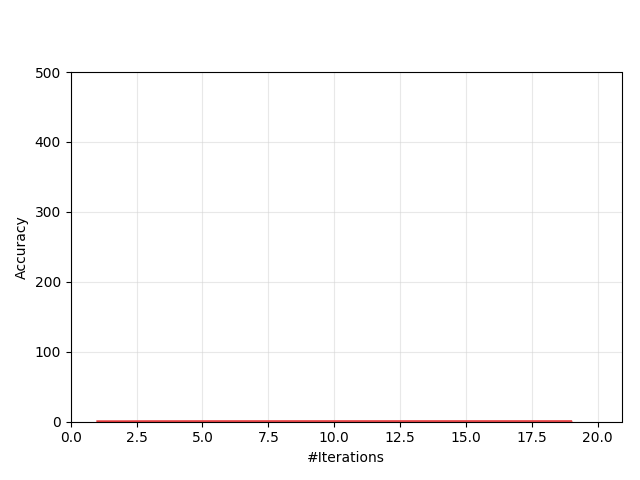
\includegraphics[height=4.5cm]{scripts/sgd_plots/train_first.png}\\
Training accuracy
\end{center}
\columnbreak
\begin{center}
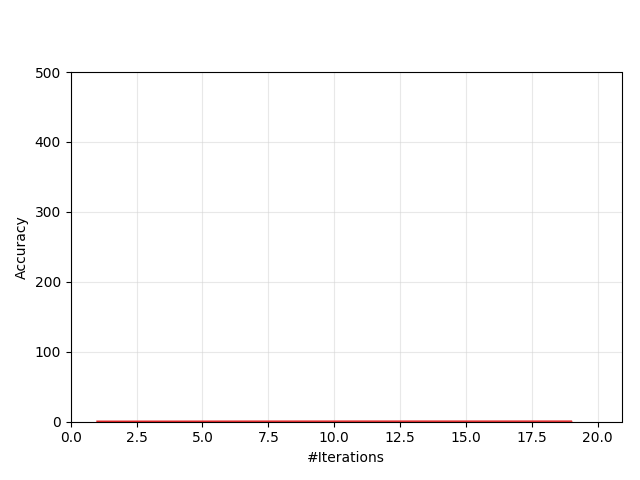
\includegraphics[height=4.5cm]{scripts/sgd_plots/test_first.png}\\
Test accuracy
\end{center}
\end{multicols}

\begin{itemize}
  \item \alert{Learning curve}: accuracy as a function of time
\end{itemize}
  
\end{frame}
%-----------------------------------------------------------------------

%----------------------------------------------------------------------
\begin{frame}[c]{Stochastic gradient descent: many learning curves}


\begin{multicols}{2}
\begin{center}
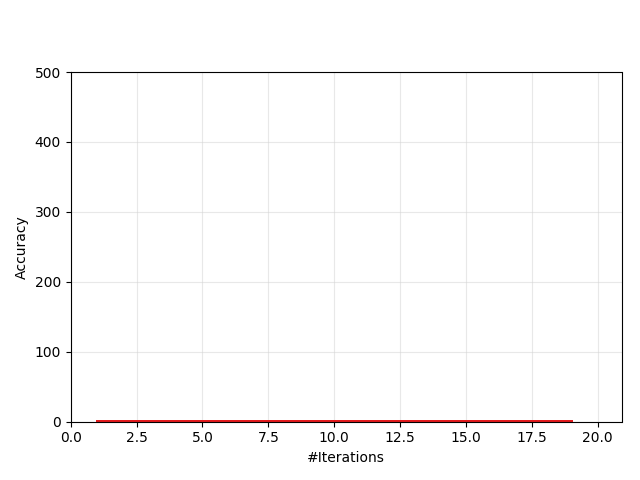
\includegraphics[height=4.5cm]{scripts/sgd_plots/train_all.png}\\
Training accuracy
\end{center}
\columnbreak
\begin{center}
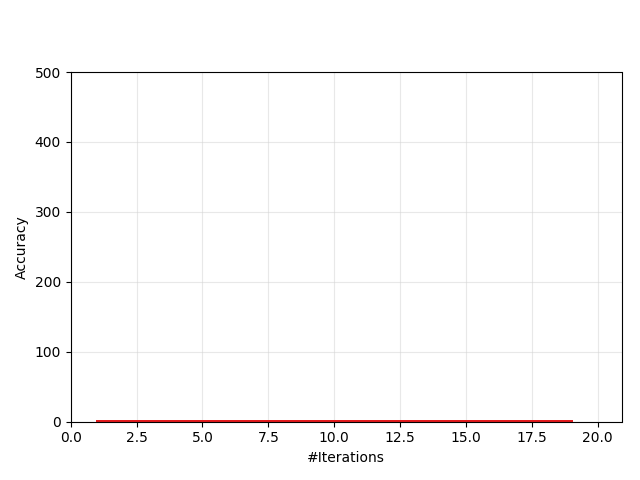
\includegraphics[height=4.5cm]{scripts/sgd_plots/test_all.png}\\
Test accuracy
\end{center}
\end{multicols}

%\begin{itemize}
%  \item Performance in a single representative run
%\end{itemize}
  
\end{frame}
%-----------------------------------------------------------------------


%----------------------------------------------------------------------
\begin{frame}[c]{Stochastic gradient descent: distribution of learning curves}


\begin{multicols}{2}
\begin{center}
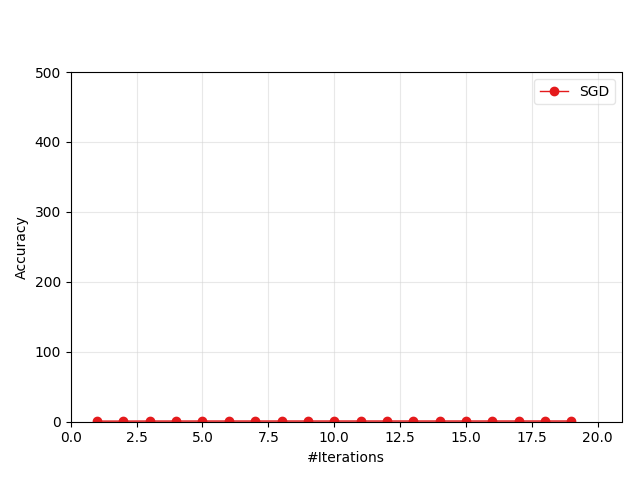
\includegraphics[height=4.5cm]{scripts/sgd_plots/train_mean.png}\\
Training accuracy
\end{center}
\columnbreak
\begin{center}
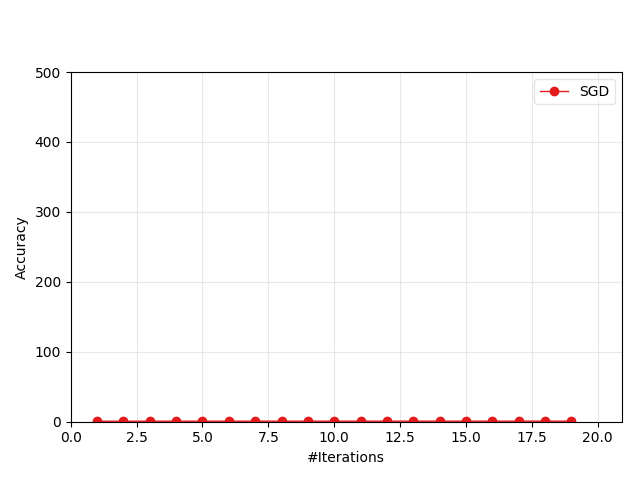
\includegraphics[height=4.5cm]{scripts/sgd_plots/test_mean.png}\\
Test accuracy
\end{center}
\end{multicols}

%\begin{itemize}
%  \item Performance in a single representative run
%\end{itemize}
  
\end{frame}
%-----------------------------------------------------------------------

%----------------------------------------------------------------------
\begin{frame}[c]{Stochastic gradient descent: different
hyperparameters}


\begin{multicols}{2}
\begin{center}
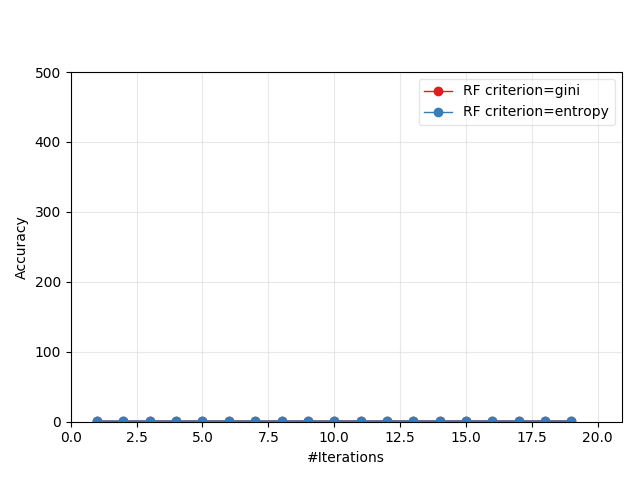
\includegraphics[height=4cm]{scripts/sgd_plots/train_mean_comparison.png}\\
Training accuracy
\end{center}
\columnbreak
\begin{center}
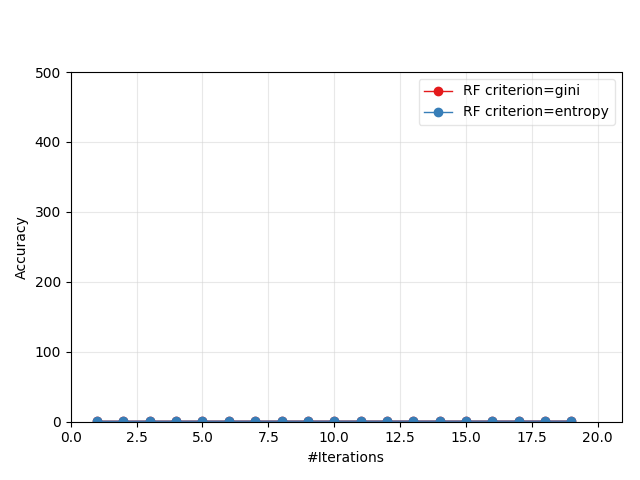
\includegraphics[height=4cm]{scripts/sgd_plots/test_mean_comparison.png}\\
Test accuracy
\end{center}
\end{multicols}

\begin{itemize}
  \item Most important hyperparameter: \alert{initial learning rate} $\eta_0$
\end{itemize}
  
\end{frame}
%-----------------------------------------------------------------------

%----------------------------------------------------------------------
\begin{frame}[c]{Qualified runtime distributions}


\begin{center}
\includegraphics[height=4cm]{scripts/sgd_plots/eta0001_eta0002_cdf.png}\\
\end{center}

\begin{itemize}
  \item Distributions of runtime \alert{to reach a specified solution quality}\\
  (here, 0.62)
\end{itemize}
  
\end{frame}
%-----------------------------------------------------------------------

%----------------------------------------------------------------------
\begin{frame}[c]{Boxplots and statistical tests}

\begin{center}
\includegraphics[height=4cm]{scripts/sgd_plots/eta0001_eta0002_boxplot.pdf}\\
\end{center}

\begin{itemize}
  \item Runtime to obtain accuracy of 0.62
  \item Difference statistically significant\\
  (unpaired permutation test, p-value 0.0000)
\end{itemize}
  
\end{frame}
%-----------------------------------------------------------------------

%----------------------------------------------------------------------
\begin{frame}[c]{Summary: Learning Goals}

After this lecture, you are able to \ldots

\begin{itemize}
  \item explain how computer science (CS) differs from other empirical sciences
  \item compare performances of algorithms by using \alert{visualization techniques}
  \begin{itemize}
    \item tabular comparison
    \item runtime distributions
    \item scatter plots
    \item box plots
  \end{itemize}
  \item explain how \alert{statistical tests} can be used 
  \item \alert{apply all these techniques} to algorithms from hard combinatorial optimizations and machine learning
\end{itemize}

\end{frame}
%-----------------------------------------------------------------------